\documentclass[a4paper,12pt]{article}

% Font
\usepackage[T1]{fontenc}
\usepackage{gentium}

% Math packages
\usepackage{amsmath}
\usepackage{amsfonts}
\usepackage{amssymb}
\usepackage{amsthm}
\usepackage{bm}

% Define symbol shortcuts
\newcommand{\cc}{\mathcal{C}}
\newcommand{\dd}{\mathcal{D}}
\newcommand{\hh}{\mathcal{H}}
\newcommand{\xx}{{\bm x}}
\newcommand{\yy}{{\bm y}}
\newcommand{\ww}{{\bm w}}

% Math environment
\newtheorem*{thm}{Theorem}

% Better list management:
% - vertical spacing in lists
% - items in lists start with dash not bullet point.
\usepackage{enumitem}
\setlist{label=\textemdash,
  itemsep=0pt, topsep=3pt, partopsep=0pt} 

% Include graphics
\usepackage{graphicx}
\usepackage{subcaption}

% Page format 
\usepackage[top=2cm,left=2cm,right=2cm,bottom=2cm]{geometry}

\begin{document}
%%% HEADER
\raisebox{0.6in}[0in]{\makebox[\textwidth][r]{\it Unproofed version }}
\vspace{-0.7in}

\begin{center}
\bf\large MA2823: Foundations of Machine Learning \\
Chapter 10: Artificial Neural Networks
\end{center}

\noindent
Lecturer: Chlo\'e-Agathe Azencott   
\hfill
Scribe: Meryll Dindin, Horace Guy

\noindent
\rule{\textwidth}{1pt}

\medskip

%%% NOTES START HERE

\section{Introduction to human brain :}

\indent
The motivation of neural networks comes from the humain brain. Our brain is made out of neurons, communicating through axones ($10^{10}$ neurons and $10^4$ connections). We recognize the advantages of parallel processing, distributed computation and memory, but it is also all about a robust system to noise and failures. To classify pictures thanks to a neural network will work the same way as our brain does, to identify features and be able to recognize the same time of pictures afterwards.

\section{Perceptron}

\indent
The model of perceptron has been introduced in 1958 thanks to Rosenblatt. The model presents layers : a labeled input, weighted connections and an output. It is a {\bfseries parametric model}, since we know, before running the model, the shape of the model. Here it is a linear combination of the defined weights for each connection. 

\vspace{0.1in}

\centerline{The model function looks like : $f(\xx) = \sum_{j=1}^p w_j x_j + w_0 = \ww^T \cdot \xx$ }

\vspace{0.1in}

\indent
Concerning the shape of the decision boundary, it is a {\bfseries hyperplane}, as it is the case for {\itshape linear regression}. If we now want to output the probability of belonging to the positive class, we apply a {\bfseries logistic function}. An example of it is the {\itshape sigmoid function} defined below :

\[\sigma(u) = \frac{1}{1+exp(-u)}\]

\begin{figure}[!ht]
\centerline{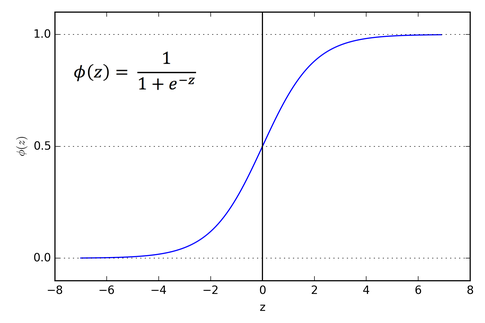
\includegraphics[width=0.5\textwidth]{./figures/sigmoid_fun.png}}
\end{figure}

\indent 
To conclude with a short summary : 
\begin{itemize}
	\item Regression : \[f(\xx) = \ww \cdot \xx + w_0\]
	\item Classification : \[ f(\xx) = s( \ww ^T\xx) = s (w_0 + \sum_{j=1}^p w_j x_j ) \]
knowing $s(o(\xx)) = \mathbb{I}_{o(\xx) > 0}$
\end{itemize}

\begin{figure}[!ht]
\centerline{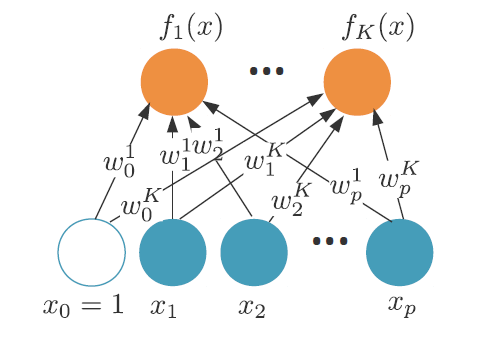
\includegraphics[width=0.5\textwidth]{./figures/multicl_1lay_per.png}}
\end{figure}
\centerline{\footnotesize{Multi-Class One Layer Perceptron}}

\vspace{0.1in}

\indent
For multiclass classification, the model is similar except for the specificity that we will rather use K output units. For each class, we reason as a binary decision (does it belong to the class or not). To get probabilities, you may use the {\bfseries softmax} function, which is similar to the maximum, except that it is differentiable. If the output for one class is sufficiently larger than for the others, its softmax output will be close to 1.

\vspace{0.1in}

\[  f_k(\xx) =  \frac{\exp(o_k)}{\sum_{l=1}^K \exp(o_l)} \text{ with } o_k = \ww ^{kT} \cdot \xx \]

Then we choose the class $C_k$ if $f_k(\xx) = \max_{l \in [1,K]} f_l(\xx) $
\section{Training a perceptron}

\indent
You generally have two possibilities : {\bfseries online learning}, which roam every instances one by one, and the {\bfseries batch learning}, that consider all the data-set in a whole. It is a flexible model, that may adapt to a changing problem over time. As a consequence comes the {\bfseries generic update rule} which means that everytime we have a new training instance, each weight get updated, taking into account the previously established weights $w_j \leftarrow w_j + \Delta w_j $. The update term can be computed as follow, knowing the error function $Error(f(\xx^i),y^i)$ and setting (arbitrary) the \emph{learning rate} $\eta$ :

\[ \Delta w_j = - \eta \frac{\partial Error(f(\xx^i), y^i)}{\partial w_j} \]

We will see that in each of the following cases, which present different error functions, this expression simplifies to the same form :

\[ \Delta w_j = \eta (y^i - f(\xx^i) ) x_j^i \]

\vspace{0.1in}

\paragraph*{Regression}
Having $Error(f(\xx^i),y^i) = \frac{1}{2} (y^i - f(\xx^i))^2 = \frac{1}{2} (y^i - \ww ^T \xx^i)^2$, that leads to the above-stated formula.

\paragraph*{Classification}
We introduce the sigmoid output $\sigma (u) = \frac{1}{1 + \exp(-u)}$ which derives as $\sigma'(u) = u'\sigma (u) (1 - \sigma(u))$ ; $f$ expresses then as $f(\xx^i) = \sigma (\ww^T\xx^i) $. 
We then use the cross-entropy error, which has the same purpose than the error function established for the regression case 

\[ Error(f(\xx^i), y^i) = -y^i \log f(\xx^i) - (1-y^i) \log (1-f(\xx^i)) \]

\paragraph*{K classes} 
With the definition of the softmax outputs stated in section 2, we can compute the Cross-entropy error :
\[ Error(f(\xx^i), y^i) = - \sum_{k=1}^K y_k^i \log f_k(\xx^i) \]


\indent
We observe that the generic rule for regression is exactly the same than for the classification model. To make it simple : the update rule is equal to the learning rate times the difference between the desired output and the actual output times the input. It comes to mind that if the desired output is equal to the actual output, there will be no change. But if they're not, the predictions will get less accurate.

\indent
Still, it has limitations. It can learn the logical AND but not the logical XOR (because data cannot be separated by a hyperplane). This is considered as a very limitated model.


\begin{figure}[!ht]
\centerline{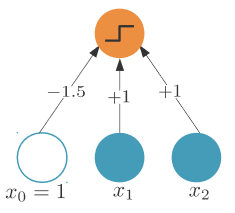
\includegraphics[width=0.4\textwidth]{./figures/perceptron_AND.png}}
\end{figure}
\centerline{\footnotesize{Learning of the logical operator AND, with a single layer perceptron.}}
\vspace{0.1in}

\indent
To quote Minsky and Papert in 1969 : {\itshape"The perceptron has shown itself worthy of study despite (and even because of!) its severe limitations. It has many features to attract attention: its linearity; its intriguing learning theorem; its clear paradigmatic simplicity as a kind of parallel computation. There is no reason to suppose that any of these virtues carry over to the many-layered version. Nevertheless, we consider it to be an important research problem to elucidate (or reject) our intuitive judgement that the extension to multilayer systems is sterile."}

\section{Multilayer Perceptrons}

\indent
Every node of the hidden layer is the output of a sigmoid perceptron. Then the output of the entire model is a linear combination of the different sigmoid perceptrons, which makes it non-linear in x ! We then came from a linear model and ended up with a non-linear model. As a consequence, the logical XOR can be learned !

{\bfseries Universal Approximation :} Any continuous function on a compact subset of $\mathbb{R}^n$ can be approximated to any arbitrary degree of precision by a feed-forward multi-layer perceptron with a single hidden layer containing a finite number of neurons.

\newpage

\begin{figure}[!ht]
\centerline{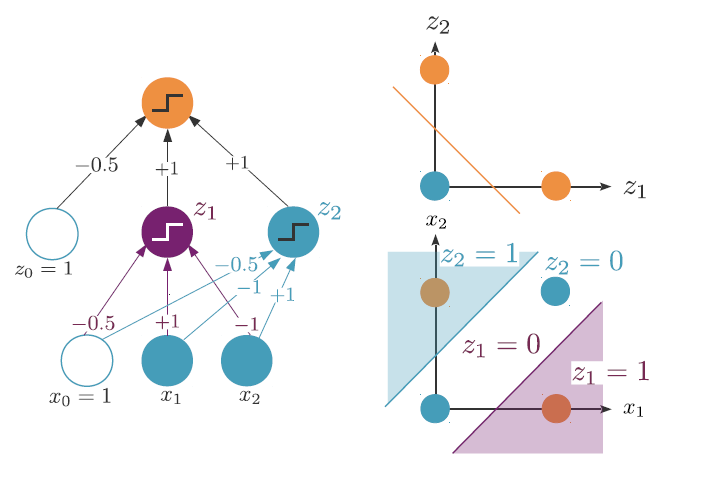
\includegraphics[width=0.7\textwidth]{./figures/XOR_learn.png}}
\end{figure}
\centerline{\footnotesize{Learning of the logical operator XOR.}}

\vspace{0.1in}

\subsection{Backpropagation}

\indent
This is one of the most powerful tool in deep-learning. The question of who invented it is still being discussed. 

\vspace{0.1in}

\indent
Backpropagation, an abbreviation for "backward propagation of errors", is a common method of training artificial neural networks used in conjunction with an optimization method such as gradient descent. It calculates the gradient of a loss function with respect to all the weights in the network, so that the gradient is fed to the optimization method which in turn uses it to update the weights, in an attempt to minimize the loss function.

\vspace{0.1in}

{\itshape Source : https://en.wikipedia.org/wiki/Backpropagation}

\vspace{0.1in}

\indent
This method may be used for binary model or multiclass perceptron. The mathematics hidden behind this process may be summed up in the following lines :

\[ z_h = \frac{1}{1+e^{- \ww_h^T \cdot \xx}}\]
\[ f(\xx) = v^T \cdot \xx = v_0 + \sum_{h=1}^H \frac{v_h}{1+e^{- \ww_h^T \cdot \xx}} \]
\[ \frac{\partial E}{\partial w_{h_j}} = \frac{\partial E}{\partial f(\xx)} \cdot \frac{\partial f(\xx)}{\partial z_h} \cdot \frac{\partial z_h}{\partial  w_{h_j}} \]

\vspace{0.1in}

\indent
Concerning the generic update rule, we obtain, thanks to the previously exposed formulas the next updated weights :

\begin{itemize}
\item {\bfseries Regression :}
\[ \Delta w_{jh} = -\eta \frac{\partial E^i}{\partial w_{jh}} = -\eta (y^i - f(\xx^i)) v_h z_h^i (1 - z_h^i) x_j^i \]
\item {\bfseries Classification :}
\[ \Delta w_{jh} = - \eta \frac{\partial E^i}{\partial w_{jh}} = \eta \sum_{i=1}^n (y^i - f(\xx^i)) v_h z_h^i (1 - z_h^i) x_j^i \]
\item {\bfseries K Classes :}
\[ \Delta w_{jh} = - \eta \frac{\partial E^i}{\partial w_{jh}} = \eta \sum_{i=1}^n \left( \sum_{k=1}^K (y_k^i - f_k(\xx^i)) v_{kh} \right) z_h^i (1 - z_h^i) x_j^i \]
\end{itemize}

\subsection{Deep-Learning}

\indent
Deep-learning can then be introduced thanks to hidden multilayers perceptrons. The more the hidden layers, the more complex and 'deep' is the learning.

\section{Neural Network Magic}

\indent 
The architecture is the following : Start with one hidden layer, stop adding layers when you're overfitting, never use more weights than training samples ! Concerning the {\bfseries weight sharing}, different units may have connections to different inputs but may be sharing the same weights. Another flexibility remain in modifying the {\bfseries network size}, in a destructive or constructive way, as much as {\bfseries overtraining} is.

\begin{figure}[!ht]
\centerline{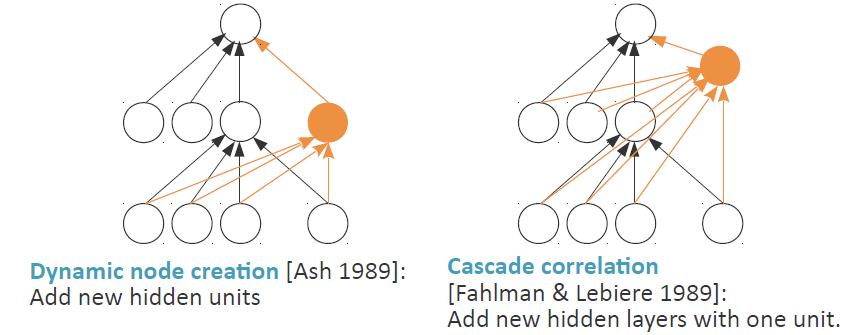
\includegraphics[width=0.7\textwidth]{./figures/growing_netw.png}}
\end{figure}
\centerline{\footnotesize{Growing network until satisfactory error rate is reached.}}

\vspace{0.1in}

\indent
There exist a lot of optimization algorithms : {\bfseries Batch Learning} where the weights are updated after a complete pass over the training set, {\bfseries Mini-Batch Learning} where the weights are updates after a pass over a set of training points of fixed size, Quasi-Newton Methods (Levenberg-Marquardt), Conjugate Gradient Descent, ... But still, {\bfseries neural newtorks are hard to train}, and they imply a lot of methods to be implemented, such as {\itshape preconditionning} that standardizes inputs and targets, initializes weights carefully to avoid saturation (implied by large weigths) and uses local learning rates

\subsection{For fun :}

Playing with a neural network : 
\vspace{0.1in}
\centerline{http://playground.tensorflow.org/}
\vspace{0.1in}

\end{document}
